\documentclass{standalone}
\usepackage{tikz}
\usetikzlibrary{patterns, positioning}

\begin{document}
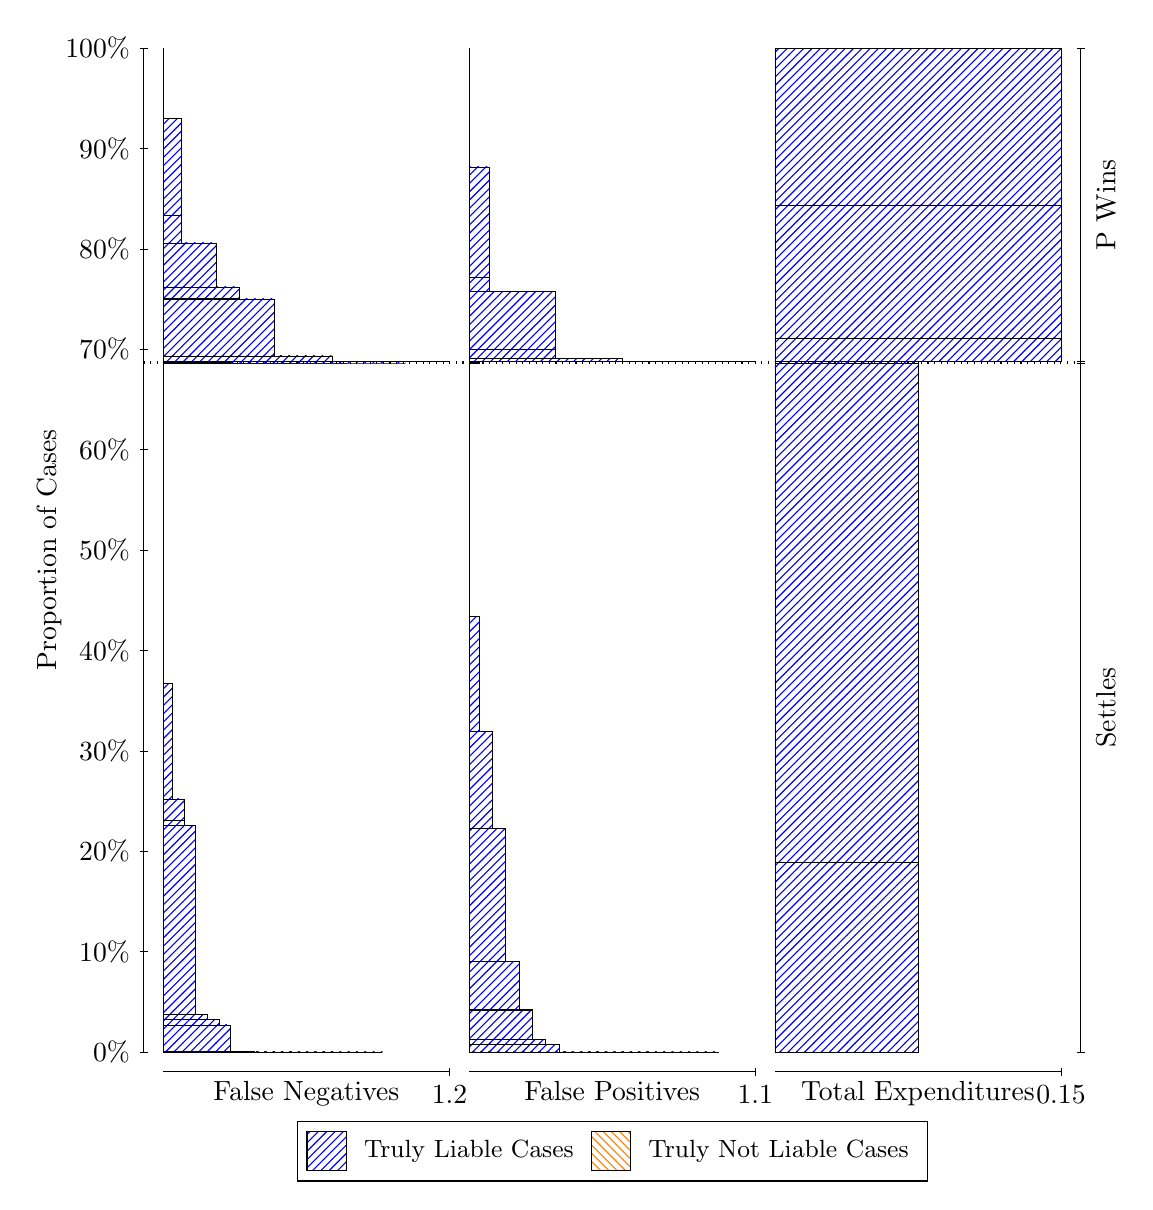
\begin{tikzpicture}
\draw[black, very thin] (1.5,1.75) -- (1.5,14.5);
\node[rotate=90, anchor=center] at (0.3, 8.125) {Proportion of Cases};
\draw[black, very thin] (1.45,1.75) -- (1.55,1.75);
\node[anchor=east] at (1.45, 1.75) {0\%};
\draw[black, very thin] (1.45,3.025) -- (1.55,3.025);
\node[anchor=east] at (1.45, 3.025) {10\%};
\draw[black, very thin] (1.45,4.3) -- (1.55,4.3);
\node[anchor=east] at (1.45, 4.3) {20\%};
\draw[black, very thin] (1.45,5.575) -- (1.55,5.575);
\node[anchor=east] at (1.45, 5.575) {30\%};
\draw[black, very thin] (1.45,6.85) -- (1.55,6.85);
\node[anchor=east] at (1.45, 6.85) {40\%};
\draw[black, very thin] (1.45,8.125) -- (1.55,8.125);
\node[anchor=east] at (1.45, 8.125) {50\%};
\draw[black, very thin] (1.45,9.4) -- (1.55,9.4);
\node[anchor=east] at (1.45, 9.4) {60\%};
\draw[black, very thin] (1.45,10.675) -- (1.55,10.675);
\node[anchor=east] at (1.45, 10.675) {70\%};
\draw[black, very thin] (1.45,11.95) -- (1.55,11.95);
\node[anchor=east] at (1.45, 11.95) {80\%};
\draw[black, very thin] (1.45,13.225) -- (1.55,13.225);
\node[anchor=east] at (1.45, 13.225) {90\%};
\draw[black, very thin] (1.45,14.5) -- (1.55,14.5);
\node[anchor=east] at (1.45, 14.5) {100\%};

\draw[black, very thin] (13.4,1.75) -- (13.4,14.5);
\draw[black, very thin] (13.35,1.75) -- (13.45,1.75);
\node[anchor=west] at (13.35, 1.75) {};
\draw[black, very thin] (13.35,10.5) -- (13.45,10.5);
\node[anchor=west] at (13.35, 10.5) {};
\draw[black, very thin] (13.35,10.517) -- (13.45,10.517);
\node[anchor=west] at (13.35, 10.517) {};
\draw[black, very thin] (13.35,14.5) -- (13.45,14.5);
\node[anchor=west] at (13.35, 14.5) {};

\draw[black, very thin, pattern color=blue, pattern=north east lines] (1.75,1.75) rectangle (4.5306,1.75);
\draw[black, very thin, pattern color=blue, pattern=north east lines] (1.75,1.75) rectangle (4.234,1.75);
\draw[black, very thin, pattern color=blue, pattern=north east lines] (1.75,1.75) rectangle (3.9374,1.75);
\draw[black, very thin, pattern color=blue, pattern=north east lines] (1.75,1.75) rectangle (3.7891,1.75);
\draw[black, very thin, pattern color=blue, pattern=north east lines] (1.75,1.75) rectangle (3.6408,1.75);
\draw[black, very thin, pattern color=blue, pattern=north east lines] (1.75,1.75) rectangle (3.4925,1.75);
\draw[black, very thin, pattern color=blue, pattern=north east lines] (1.75,1.75) rectangle (3.3442,1.7508);
\draw[black, very thin, pattern color=blue, pattern=north east lines] (1.75,1.7508) rectangle (3.1959,1.7508);
\draw[black, very thin, pattern color=blue, pattern=north east lines] (1.75,1.7508) rectangle (3.0476,1.7508);
\draw[black, very thin, pattern color=blue, pattern=north east lines] (1.75,1.7508) rectangle (2.8993,1.7537);
\draw[black, very thin, pattern color=blue, pattern=north east lines] (1.75,1.7537) rectangle (2.751,1.7575);
\draw[black, very thin, pattern color=blue, pattern=north east lines] (1.75,1.7575) rectangle (2.6027,2.0954);
\draw[black, very thin, pattern color=blue, pattern=north east lines] (1.75,2.0954) rectangle (2.4544,2.1602);
\draw[black, very thin, pattern color=blue, pattern=north east lines] (1.75,2.1602) rectangle (2.3061,2.2291);
\draw[black, very thin, pattern color=blue, pattern=north east lines] (1.75,2.2291) rectangle (2.1578,4.6318);
\draw[black, very thin, pattern color=blue, pattern=north east lines] (1.75,4.6318) rectangle (2.0095,4.6951);
\draw[black, very thin, pattern color=blue, pattern=north east lines] (1.75,4.6951) rectangle (2.0095,4.9646);
\draw[black, very thin, pattern color=blue, pattern=north east lines] (1.75,4.9646) rectangle (1.8612,6.427);
\draw[black, very thin, pattern color=orange, pattern=north west lines] (1.75,6.427) rectangle (1.75,6.427);
\draw[black, very thin, pattern color=blue, pattern=north east lines] (1.75,6.427) rectangle (1.75,10.5);
\draw[black, very thin, pattern color=blue, pattern=north east lines] (1.75,10.5) rectangle (4.8272,10.5);
\draw[black, very thin, pattern color=blue, pattern=north east lines] (1.75,10.5) rectangle (4.0857,10.5);
\draw[black, very thin, pattern color=blue, pattern=north east lines] (1.75,10.5) rectangle (3.3442,10.5);
\draw[black, very thin, pattern color=blue, pattern=north east lines] (1.75,10.5) rectangle (2.6027,10.507);
\draw[black, very thin, pattern color=blue, pattern=north east lines] (1.75,10.507) rectangle (1.8612,10.517);
\draw[black, very thin, pattern color=orange, pattern=north west lines] (1.75,10.517) rectangle (1.75,10.517);
\draw[black, very thin, pattern color=blue, pattern=north east lines] (1.75,10.517) rectangle (5.3833,10.517);
\draw[black, very thin, pattern color=blue, pattern=north east lines] (1.75,10.517) rectangle (4.6418,10.518);
\draw[black, very thin, pattern color=blue, pattern=north east lines] (1.75,10.518) rectangle (4.1969,10.518);
\draw[black, very thin, pattern color=blue, pattern=north east lines] (1.75,10.518) rectangle (3.9003,10.589);
\draw[black, very thin, pattern color=blue, pattern=north east lines] (1.75,10.589) rectangle (3.4554,10.589);
\draw[black, very thin, pattern color=blue, pattern=north east lines] (1.75,10.589) rectangle (3.1588,11.315);
\draw[black, very thin, pattern color=blue, pattern=north east lines] (1.75,11.315) rectangle (2.7139,11.319);
\draw[black, very thin, pattern color=blue, pattern=north east lines] (1.75,11.319) rectangle (2.7139,11.466);
\draw[black, very thin, pattern color=blue, pattern=north east lines] (1.75,11.466) rectangle (2.4173,12.026);
\draw[black, very thin, pattern color=blue, pattern=north east lines] (1.75,12.026) rectangle (1.9724,12.377);
\draw[black, very thin, pattern color=blue, pattern=north east lines] (1.75,12.377) rectangle (1.9724,13.611);
\draw[black, very thin, pattern color=orange, pattern=north west lines] (1.75,13.611) rectangle (1.75,13.611);
\draw[black, very thin, pattern color=blue, pattern=north east lines] (1.75,13.611) rectangle (1.75,14.5);
\draw[black, very thin, pattern color=orange, pattern=north west lines] (5.6333,1.75) rectangle (8.8019,1.75);
\draw[black, very thin, pattern color=blue, pattern=north east lines] (5.6333,1.75) rectangle (8.8019,1.75);
\draw[black, very thin, pattern color=orange, pattern=north west lines] (5.6333,1.75) rectangle (8.126,1.75);
\draw[black, very thin, pattern color=blue, pattern=north east lines] (5.6333,1.75) rectangle (8.126,1.75);
\draw[black, very thin, pattern color=blue, pattern=north east lines] (5.6333,1.75) rectangle (7.957,1.75);
\draw[black, very thin, pattern color=orange, pattern=north west lines] (5.6333,1.75) rectangle (7.788,1.75);
\draw[black, very thin, pattern color=blue, pattern=north east lines] (5.6333,1.75) rectangle (7.788,1.75);
\draw[black, very thin, pattern color=orange, pattern=north west lines] (5.6333,1.75) rectangle (7.45,1.75);
\draw[black, very thin, pattern color=blue, pattern=north east lines] (5.6333,1.75) rectangle (7.45,1.75);
\draw[black, very thin, pattern color=blue, pattern=north east lines] (5.6333,1.75) rectangle (7.281,1.75);
\draw[black, very thin, pattern color=orange, pattern=north west lines] (5.6333,1.75) rectangle (7.112,1.75);
\draw[black, very thin, pattern color=blue, pattern=north east lines] (5.6333,1.75) rectangle (7.112,1.7513);
\draw[black, very thin, pattern color=blue, pattern=north east lines] (5.6333,1.7513) rectangle (6.943,1.7513);
\draw[black, very thin, pattern color=orange, pattern=north west lines] (5.6333,1.7513) rectangle (6.774,1.7513);
\draw[black, very thin, pattern color=blue, pattern=north east lines] (5.6333,1.7513) rectangle (6.774,1.8421);
\draw[black, very thin, pattern color=blue, pattern=north east lines] (5.6333,1.8421) rectangle (6.605,1.906);
\draw[black, very thin, pattern color=orange, pattern=north west lines] (5.6333,1.906) rectangle (6.436,1.906);
\draw[black, very thin, pattern color=blue, pattern=north east lines] (5.6333,1.906) rectangle (6.436,2.2857);
\draw[black, very thin, pattern color=blue, pattern=north east lines] (5.6333,2.2857) rectangle (6.436,2.2881);
\draw[black, very thin, pattern color=blue, pattern=north east lines] (5.6333,2.2881) rectangle (6.2671,2.9029);
\draw[black, very thin, pattern color=orange, pattern=north west lines] (5.6333,2.9029) rectangle (6.0981,2.9029);
\draw[black, very thin, pattern color=blue, pattern=north east lines] (5.6333,2.9029) rectangle (6.0981,4.5889);
\draw[black, very thin, pattern color=blue, pattern=north east lines] (5.6333,4.5889) rectangle (6.0981,4.5895);
\draw[black, very thin, pattern color=blue, pattern=north east lines] (5.6333,4.5895) rectangle (5.9291,5.8231);
\draw[black, very thin, pattern color=blue, pattern=north east lines] (5.6333,5.8231) rectangle (5.7601,7.2855);
\draw[black, very thin, pattern color=blue, pattern=north east lines] (5.6333,7.2855) rectangle (5.6333,10.5);
\draw[black, very thin, pattern color=orange, pattern=north west lines] (5.6333,10.5) rectangle (5.7601,10.5);
\draw[black, very thin, pattern color=blue, pattern=north east lines] (5.6333,10.5) rectangle (5.7601,10.51);
\draw[black, very thin, pattern color=blue, pattern=north east lines] (5.6333,10.51) rectangle (5.6333,10.517);
\draw[black, very thin, pattern color=orange, pattern=north west lines] (5.6333,10.517) rectangle (9.2667,10.517);
\draw[black, very thin, pattern color=blue, pattern=north east lines] (5.6333,10.517) rectangle (9.2667,10.517);
\draw[black, very thin, pattern color=orange, pattern=north west lines] (5.6333,10.517) rectangle (8.4217,10.517);
\draw[black, very thin, pattern color=blue, pattern=north east lines] (5.6333,10.517) rectangle (8.4217,10.517);
\draw[black, very thin, pattern color=orange, pattern=north west lines] (5.6333,10.517) rectangle (7.5767,10.517);
\draw[black, very thin, pattern color=blue, pattern=north east lines] (5.6333,10.517) rectangle (7.5767,10.558);
\draw[black, very thin, pattern color=orange, pattern=north west lines] (5.6333,10.558) rectangle (7.0698,10.558);
\draw[black, very thin, pattern color=blue, pattern=north east lines] (5.6333,10.558) rectangle (7.0698,10.558);
\draw[black, very thin, pattern color=orange, pattern=north west lines] (5.6333,10.558) rectangle (6.7318,10.558);
\draw[black, very thin, pattern color=blue, pattern=north east lines] (5.6333,10.558) rectangle (6.7318,10.676);
\draw[black, very thin, pattern color=blue, pattern=north east lines] (5.6333,10.676) rectangle (6.7318,11.406);
\draw[black, very thin, pattern color=orange, pattern=north west lines] (5.6333,11.406) rectangle (6.2248,11.406);
\draw[black, very thin, pattern color=blue, pattern=north east lines] (5.6333,11.406) rectangle (6.2248,11.406);
\draw[black, very thin, pattern color=blue, pattern=north east lines] (5.6333,11.406) rectangle (5.8868,11.587);
\draw[black, very thin, pattern color=blue, pattern=north east lines] (5.6333,11.587) rectangle (5.8868,12.99);
\draw[black, very thin, pattern color=orange, pattern=north west lines] (5.6333,12.99) rectangle (5.6333,12.99);
\draw[black, very thin, pattern color=blue, pattern=north east lines] (5.6333,12.99) rectangle (5.6333,14.5);
\draw[black, very thin, pattern color=orange, pattern=north west lines] (9.5167,1.75) rectangle (11.333,1.75);
\draw[black, very thin, pattern color=blue, pattern=north east lines] (9.5167,1.75) rectangle (11.333,4.1542);
\draw[black, very thin, pattern color=orange, pattern=north west lines] (9.5167,4.1542) rectangle (11.333,4.1542);
\draw[black, very thin, pattern color=blue, pattern=north east lines] (9.5167,4.1542) rectangle (11.333,10.5);
\draw[black, very thin, pattern color=orange, pattern=north west lines] (9.5167,10.5) rectangle (11.333,10.5);
\draw[black, very thin, pattern color=blue, pattern=north east lines] (9.5167,10.5) rectangle (11.333,10.517);
\draw[black, very thin, pattern color=orange, pattern=north west lines] (9.5167,10.517) rectangle (13.15,10.517);
\draw[black, very thin, pattern color=blue, pattern=north east lines] (9.5167,10.517) rectangle (13.15,10.818);
\draw[black, very thin, pattern color=orange, pattern=north west lines] (9.5167,10.818) rectangle (13.15,10.818);
\draw[black, very thin, pattern color=blue, pattern=north east lines] (9.5167,10.818) rectangle (13.15,12.507);
\draw[black, very thin, pattern color=orange, pattern=north west lines] (9.5167,12.507) rectangle (13.15,12.507);
\draw[black, very thin, pattern color=blue, pattern=north east lines] (9.5167,12.507) rectangle (13.15,14.5);
\draw[black, dotted] (1.5,10.5) -- (13.4,10.5);
\draw[black, dotted] (1.5,10.517) -- (13.4,10.517);
\draw[black, very thin] (1.75,1.5) -- (5.3833,1.5);
\node[anchor=north] at (3.5667, 1.5) {False Negatives};
\draw[black, very thin] (5.3833,1.45) -- (5.3833,1.55);
\node[anchor=north] at (5.3833, 1.45) {1.2};

\draw[black, very thin] (5.6333,1.5) -- (9.2667,1.5);
\node[anchor=north] at (7.45, 1.5) {False Positives};
\draw[black, very thin] (9.2667,1.45) -- (9.2667,1.55);
\node[anchor=north] at (9.2667, 1.45) {1.1};

\draw[black, very thin] (9.5167,1.5) -- (13.15,1.5);
\node[anchor=north] at (11.333, 1.5) {Total Expenditures};
\draw[black, very thin] (13.15,1.45) -- (13.15,1.55);
\node[anchor=north] at (13.15, 1.45) {0.15};

\node[black, centered, rotate=90] at (13.72, 6.1251) {Settles};

\node[black, centered, rotate=90] at (13.72, 12.508) {P Wins};

\draw (7.449999999999999,1.5) node[draw=none] (baseCoordinate) {};
\begin{scope}[align=center]
        \matrix[scale=0.5, draw=black, below=0.5cm of baseCoordinate, nodes={draw}, column sep=0.1cm]{
            \node[rectangle, draw, minimum width=0.5cm, minimum height=0.5cm, pattern=north east lines, pattern color=blue] {}; &
            \node[draw=none, font=\small] (B) {Truly Liable Cases}; &
            \node[rectangle, draw, minimum width=0.5cm, minimum height=0.5cm, pattern=north west lines, pattern color=orange] {}; &
            \node[draw=none, font=\small] (B) {Truly Not Liable Cases}; \\
            };
\end{scope}

\end{tikzpicture}
\end{document}